\documentclass[
  amsfonts,
  amsmath,
  tbtags,
  amssymb,
  aps,
  nobibnotes,
  prl,
  twocolumn,
]{revtex4-2}

% imports
\usepackage{appendix}[titletoc]
\usepackage[english]{babel}
\usepackage[justification=centering]{caption}
\usepackage{float}
\usepackage{graphicx}
\usepackage{hyperref}
\usepackage[utf8]{inputenc}
\usepackage{layouts}
\usepackage{optidef}
\usepackage{physics}
\usepackage{setspace}
\usepackage[labelformat=simple]{subcaption}
\usepackage{xcolor}

% configure imports
\DeclareMathOperator*{\argmin}{arg\,min}
\newcommand{\todo}[1]{\textcolor{red}{TODO: #1}}
\definecolor{darkgreen}{RGB}{46, 184, 46}
\newcommand{\half}{\frac{1}{2}}
\newcommand{\R}{\mathbb{R}}
\captionsetup[subfigure]{labelformat=empty, skip=0pt}
\restylefloat{table}
\renewcommand\thesubfigure{(\alph{subfigure})}



\begin{document}

%% TITLE
\title{Robust Quantum Optimal Control}

\author{Thomas Propson}
\email{tcpropson@uchicago.edu}
\affiliation{
  Department of Physics, University of Chicago, Chicago, Illinois 60637, USA
}

\date{\today}


%% ABSTRACT
\begin{abstract}
  This is a paper about robust quantum optimal control.
\end{abstract}

\maketitle


%% SECTION 1
\section{Introduction}
(Existing work) The leading model of universal
quantum computation is gate-based. The Quantum Optimal Control (QOC)
literature has saught to answer the question "What is the best way to construct a quantum gate?".
Analytic methods
have been demonstrated to construct quantum gates
\cite{zhang2020universal, huang2020engineering, han2020experimental,
  xu2020nonadiabatic, carlini2005quantum}.
Most methods rely on solving the time-dependent
Schroedinger equation analytically or deriving equations of motion
from a suitable Lagrangian.

Some analytical methods
have been presented to address realistic experimental constraints.
Considering the dynamical and geometric phases of state
evolution has led to methods for achieving
robustness to pure dephasing in quantum systems
\cite{xu2020nonadiabitc, han2020experimental, merrill2014progress}.
Additionally, suitable choices of bases have been demonstrated that
allow the experimentalist to infer tradeoffs in longitudinal
and pure dephasing coherence times \cite{huang2020engineering}.
To date, however, no analytical method has been presented
to construct a gate while satisfying all relevant experimental
constraints. Furthermore, most analytic methods have only
been demonstrated in the two-level approximation and become
cumbersome to solve for larger Hilbert space sizes.

Numerical quantum control techniques have developed in parallel
with the analytic frameworks. Numerical quantum control
techniques integrate the time-dependent Schroedinger
equation and use sensitivity analysis to optimize target metrics
of the quantum gate, such as fidelity
\cite{leung2017speedup,  goerz2019krotov, doria2011optimal,
  abdelhafez2019gradient, machnes2015gradient, leng2019robust}.
These techniques typically employ zeroth- or first-order
optimizers and make no garauntees of optimality.
Further, they formulate the quantum control
problem as unconstrained or use
projective gradient methods \cite{machnes2015gradient}.
The latter approach relies on constructing
bases for constraint spaces--which is not always feasible--and
may hinder convergence.

(This work) We employ the trajectory optimization
literature to formulate the quantum
optimal control problem as a constrained optimization problem.
The trajectory optimization framework allows us to handle arbitrary
constraints on the evolution of the quantum state. Additionally,
we introduce methods for constructing gates robust to longitudinal
relaxation and pure dephasing, the dominant barrier to experimentally
realizing practical quantum computing.

We study the quantum optimal control problem on the fluxonium qubit.
We outline experimentally realistic constraints and map them to
the trajectory optimization framework. For the device we study
we achieve a 1.5x increase in $T_{1}$ times.
We present two methods for achieving robustness to pure dephasing,
and compare them to existing dynamic decoupling methods. We find that 
our methods mitigate dephasing by order X over dynamic decoupling.

(Outline)  First we formulate the quantum optimal control problem
in the trajectory optimization framework. Then, we introduce the dynamics
of the fluxonium device and outline experimental considerations
relevant to gate construction. Next we outline a method for
making the optimization $T_{1}$ aware. Finally, we present
some methods for engineering robustness to pure dephasing and
compare them to existing techniques.


%% SECTION 2
\section{QOC + AL-iLQR}
(QOC Problem Statement) Here we introduce the notation
we will use throughout the paper,
review the quantum optimal control problem statement,
and introduce the trajectory optimization framework.
Quantum optimal control concerns the evolution of
a state $\ket{\psi(t)}$ governed by the time-dependent
Schroedinger equation
\begin{align}
  \partial_{t} \ket{\psi(t)} &= -\frac{i}{\hbar} H(\textbf{u}(t), t) \ket{\psi(t)}
\end{align}
The evolution is sometimes cast with $\rho(t) = \ket{\psi(t)}\bra{\psi(t)}$
and the Lindblad master equation to model the decoherence of the
state explicitly. The Hamiltonian
depends arbitrarily on the controls $\textbf{u}(t)$.

Numerical quantum optimal control techniques make
the problem tractable by discretizing the problem into $N$
time steps. Typical integration techniques rely on approximating
the analytical solution to the time-dependent Schroedinger equation
or using explicit integration methods, e.g. Runge-Kutta, of the form
\begin{align}
  \ket{\psi_{k + 1}} \approx \ket{\psi_{k}} + \partial_{t} \ket{\psi_{k}} \cdot \Delta t_{k}
\end{align}

Quantum optimal control seeks the control
parameters that minimize a functional $J(u, \ket{\psi_{N}(u)})$.
In the simplest case the functional
$J = 1 - {\lvert \braket{\psi_{f} \lvert \psi_{N}(u)} \rvert}^{2}$
which is the infidelity between the inital state evolved
to the final time step ($\ket{\psi_{N}(u)}$)
and the target state ($\ket{\psi_{f}}$). In general
$J$ is a linear combinaion of cost functions on $\ket{\psi_{N}(u)}$, e.g.
forbidden-state occupation, as well as
cost functions on $u$, e.g. the norm of the control amplitudes
\cite{leung2017speedup}.

(AL-iLQR Problem Statement) The trajectory optimization
literature solves a more general class of non-linear programs that resemble
the quantum optimal control problem. The quantum optimal control
problem is a specific case of the linear quadratic regulator (LQR).
LQR is so called because the dynamics are linear in the state and
the cost function is quadratic in the state. In the LQR formulation
the same functional is evaluated at each time step
\begin{equation}
  \begin{aligned}
    J_{\textrm{LQR}} = \tilde{x}_{N}^{T} Q_{N} \tilde{x}_{N}
    &+ \sum_{k = 0}^{N - 1} \tilde{x}_{k}^{T} Q_{k} \tilde{x}_{k} + u_{k}^{T} R_{k} u_{k}
  \end{aligned}
\end{equation}
where $\tilde{x}_{k} = x_{k} - x_{f}$ is the difference between the current
and final state and $Q_{k}, R_{k}$ are matrices that define the penalty metric.

The advantage of the LQR formulation
is that there exists a dynamic programming algorithm to compute the
optimal update to the controls $u_{k}$ at each time step.
This algorithm employs the Ricatti recursion (see Appendix).

In order to incorporate constraints into the problem we employ
the augmented lagrangian method. This method adaptively
updates the penalty of constraints
%% LEFT OFF HERE



Trajectory optimization gives us gaurantees
about our updates via Ricatti recursion
and allows us to put constraints on our cost functions.
%% This is e.q. 2 from ALTRO paper
\begin{equation}
\begin{aligned}[b]
  \min_{U:N-1 \times m} &\mathcal{L}_{N}(x_{N}, \lambda_{N}, \mu_{N})\\
  &+ \sum_{k = 1}^{N - 1} \mathcal{L}_{k}(x_{k}, u_{k}, \lambda_{k}, \mu_{k})\\
\end{aligned}
\end{equation}
\begin{equation}
\begin{aligned}[b]
  \mathcal{L}_{k}(x_{k}, &u_{k}, \lambda_{k}, \mu_{k}) =\\
  &(\lambda_{k} + \frac{1}{2}I_{\mu_{k}} c_{k}(x_{k}, u_{k}))^{T} c_{k}(x_{k}, u_{k})\\
  &+ (x_{k} - x_{f})^{T} Q (x_{k} - x_{f}) + u_{k}^{T} R u_{k}\\
\end{aligned}
\end{equation}
The important point is that there is an update step (e.q. 17 from ALTRO paper) where we send $\lambda \rightarrow \infty$
and get all of the nice convergence properties. The weights are adjusted dynamically between iterations until
all of our constraints are satisfied. The Markovian decision structure of the problem allows
us to apply differentiable dynamic programming to garauntee that the update for each control $U_{k}$ is
opimal, as apposed to the greedy updates of first-order optimizers like the naive gradient descent.

%% TODO: (?) Figure comparing update procedures


%% SECTION 3
\section{QOC on the Fluxonium}
(Fluxonium Device) In the two-level
approximation we have
\begin{align}
  H/h &= \omega_{q} \frac{\sigma_{z}}{2} + A(\Phi_{ext}) \frac{\sigma_{x}}{2}
\end{align}
This approximation is good up to the avoided crossing at $\Phi_{\textrm{ext}} = 0.35 \Phi_{0}$. We get $A$
by converting via $\bra{g} \hat{\phi} \ket{e}$.
We use the gates $X/2, Y/2, Z/2$. $X/2, Y/2$ are universal
up to an arbitrary Z rotation.
%% TODO: list device parameters

(Constraints) We want constraints on our pulses. We want pulses start and end at zero
for concatenation. We want pulses to have zero net flux to mitigate
hysteresis in flux bias lines.
%% TODO: See ref. 28 in Helin paper
We want the amplitude to be constrained
$\delta \Phi_{\textrm{ext}} \sim 0.06 \Phi_{0}$
so the two-level approximation stays valid.
We want our state to obey normalization conditions,
mitigating numerical error in simulaiton.
%% TODO: mention pulse smoothing via optimizing over 2nd derivative
%% of pulses
%% TODO: probably want to list equations for the constraints

($T_{1}$ and $T_{\phi}$ noise)
Dissipation to the thermal bath via longitudinal
relaxation ($T_{1}$) is an irreversible process
that results in information loss.
Pure dephasing ($T_{\phi}$) is a reversible process.
Dielectric loss, etc. contribute
to $T_{1}$. $1/f$ flux noise, etc. contribute to $T_{\phi}$
There is a tradeoff between $T_{1}$ and $T_{\phi}$. In the case of white
noise we have that the sum of the noise weights $W_{1}$ and $W_{\phi}$
is constant \cite{huang2020engineering}.
In our case $T_{\phi}$ is saturated at the flux
frustration point $\Phi_{\textrm{ext}} = 0.5 \Phi_{0}$
$T_{\phi}$ decreases as we move away from the flux
frustration point. Conversely, $T_{1}$ is at a minimum
around the flux frustration point $T_{1}(0.5 \Phi_{0}) = 0.315$ms,
and increases away from the flux frustration point
$T_{1}(0.43 \Phi_{0}) = 4.3$ms. Given the nature
of the decay processes and the tradeoff, we choose
to optimize the flux bias to have high time-averaged
$T_{1}$ times and employ some techniques to mitigate
$T_{\phi}$ dephasing.
%% TODO: See fig. 3 in Helin paper


%% SECTION 4
\section{Robustness to $T_{1}$-type Noise}
(Strategy) We seek to minimize the probability
that the qubit relaxes longitudinally.
To this end we augment the state vector $x_{k}$ with the
longitudinal relaxation probability
\begin{align}
  P_{1}(t_{k}) = \int_{0}^{t_{k}}
  \gamma_{1}(\Phi_{\textrm{ext}}(t)) dt
\end{align}
where $\gamma_{1} = T_{1}^{-1}$. Setting the target
longitudinal relaxation probability to 0 results in
a quadratic cost at each knot point
of the form ${\lvert P_{1}(t_{k}) \rvert}^{2}$.

The value $T_{1}(\Phi_{\textrm{ext}}(t_{k}))$
is obtained at each knot point by evaluating
a spline interpolant fit to
experimentally obtained data of the form
$\{(\Phi_{\textrm{ext}}, T_{1})\}$.
Calculating $T_{1}$ directly from theoretical
considerations requires many high-dimensional
eigendecompositions, which
is computationally expensive. Additionally,
$T_{1}$ values are known to fluctuate greatly
with laboratory temperatures \cite{klimov2018fluctuations}.
Interpolating $T_{1}$ from experimental data increases
the fridge truth of the simulation.

Furthermore, the probability of longitudinal 
relaxation is dependent on the gate duration $t_{N}$.
We allow the optimizer to tune the gate duration by
augmenting the control vector $u_{k}$ with
the time step between knot points $\Delta t_{k}$.
Promoting $\Delta t_{k}$ to a decision variable, rather
than the number of knot points $N$, preserves the
Markovian decision structure of the trajectory
optimization problem. To ensure numerical
integration accuracy is maintained we add a bound
constraint at each knot point
$5\textrm{e-}3 \ \textrm{ns} \le
\Delta t_{k} \le 2\textrm{e-}2 \ \textrm{ns}$.
Note that this bound constraint is allowed to be
broken for intermediate iterations of the optimization,
so we use the absolute value of the time step
$\lvert \Delta t_{k} \rvert$ to ensure that it is non-negative.

(Results) We achieve a factor of 1.5 decrease in the probability
of longitudinal relaxation from the analytic gates we benchmark
against. We simulate the performance of the gates using the
lindblad master equation (see Appendix X). We repeatedly apply the basis gates
and measure the fidelity of the resulting state as a function
of time as shown in Fig. 1.

%% T4.1
%% TODO: Update this table with spline T1 optimizations and calculations.
%% TODO: Maybe best for appendix.
%% TOOD: Maybe add some commentary about why we see more speedup
%% for Z/2 and X/2 than Y/2. In particular I think this is because of the
%% long idle times at the flux frustration point for Z/2 and X/2. It
%% might be a more fair comparison to show gates that have better T1s
%% and as good flux noise mitigation.
\begin{table}
  \begin{tabular}{c | c | c | c}
    & Analytic  & QOC &\\
    Gate & $P_{1}\ (10^{-5})$ & $P_{1}\ (10^{-5})$ & Speedup\\
    \hline
    Z/2 & 4.615 & 2.576 & 1.792\\
    Y/2 & 2.826 & 1.888 & 1.496\\
    X/2 & 9.562 & 5.080 & 1.882\\
  \end{tabular}
  \caption{Probability of longitudinal relaxation for each gate
    evaluated at the gate's duration.}
\end{table}


%% F4.1
%% TODO: Update images. Use new gates constructed with
%% spline T1 and use smaller sim times.
\begin{figure}[ht]
  \begin{subfigure}{.33\textwidth}
    %% 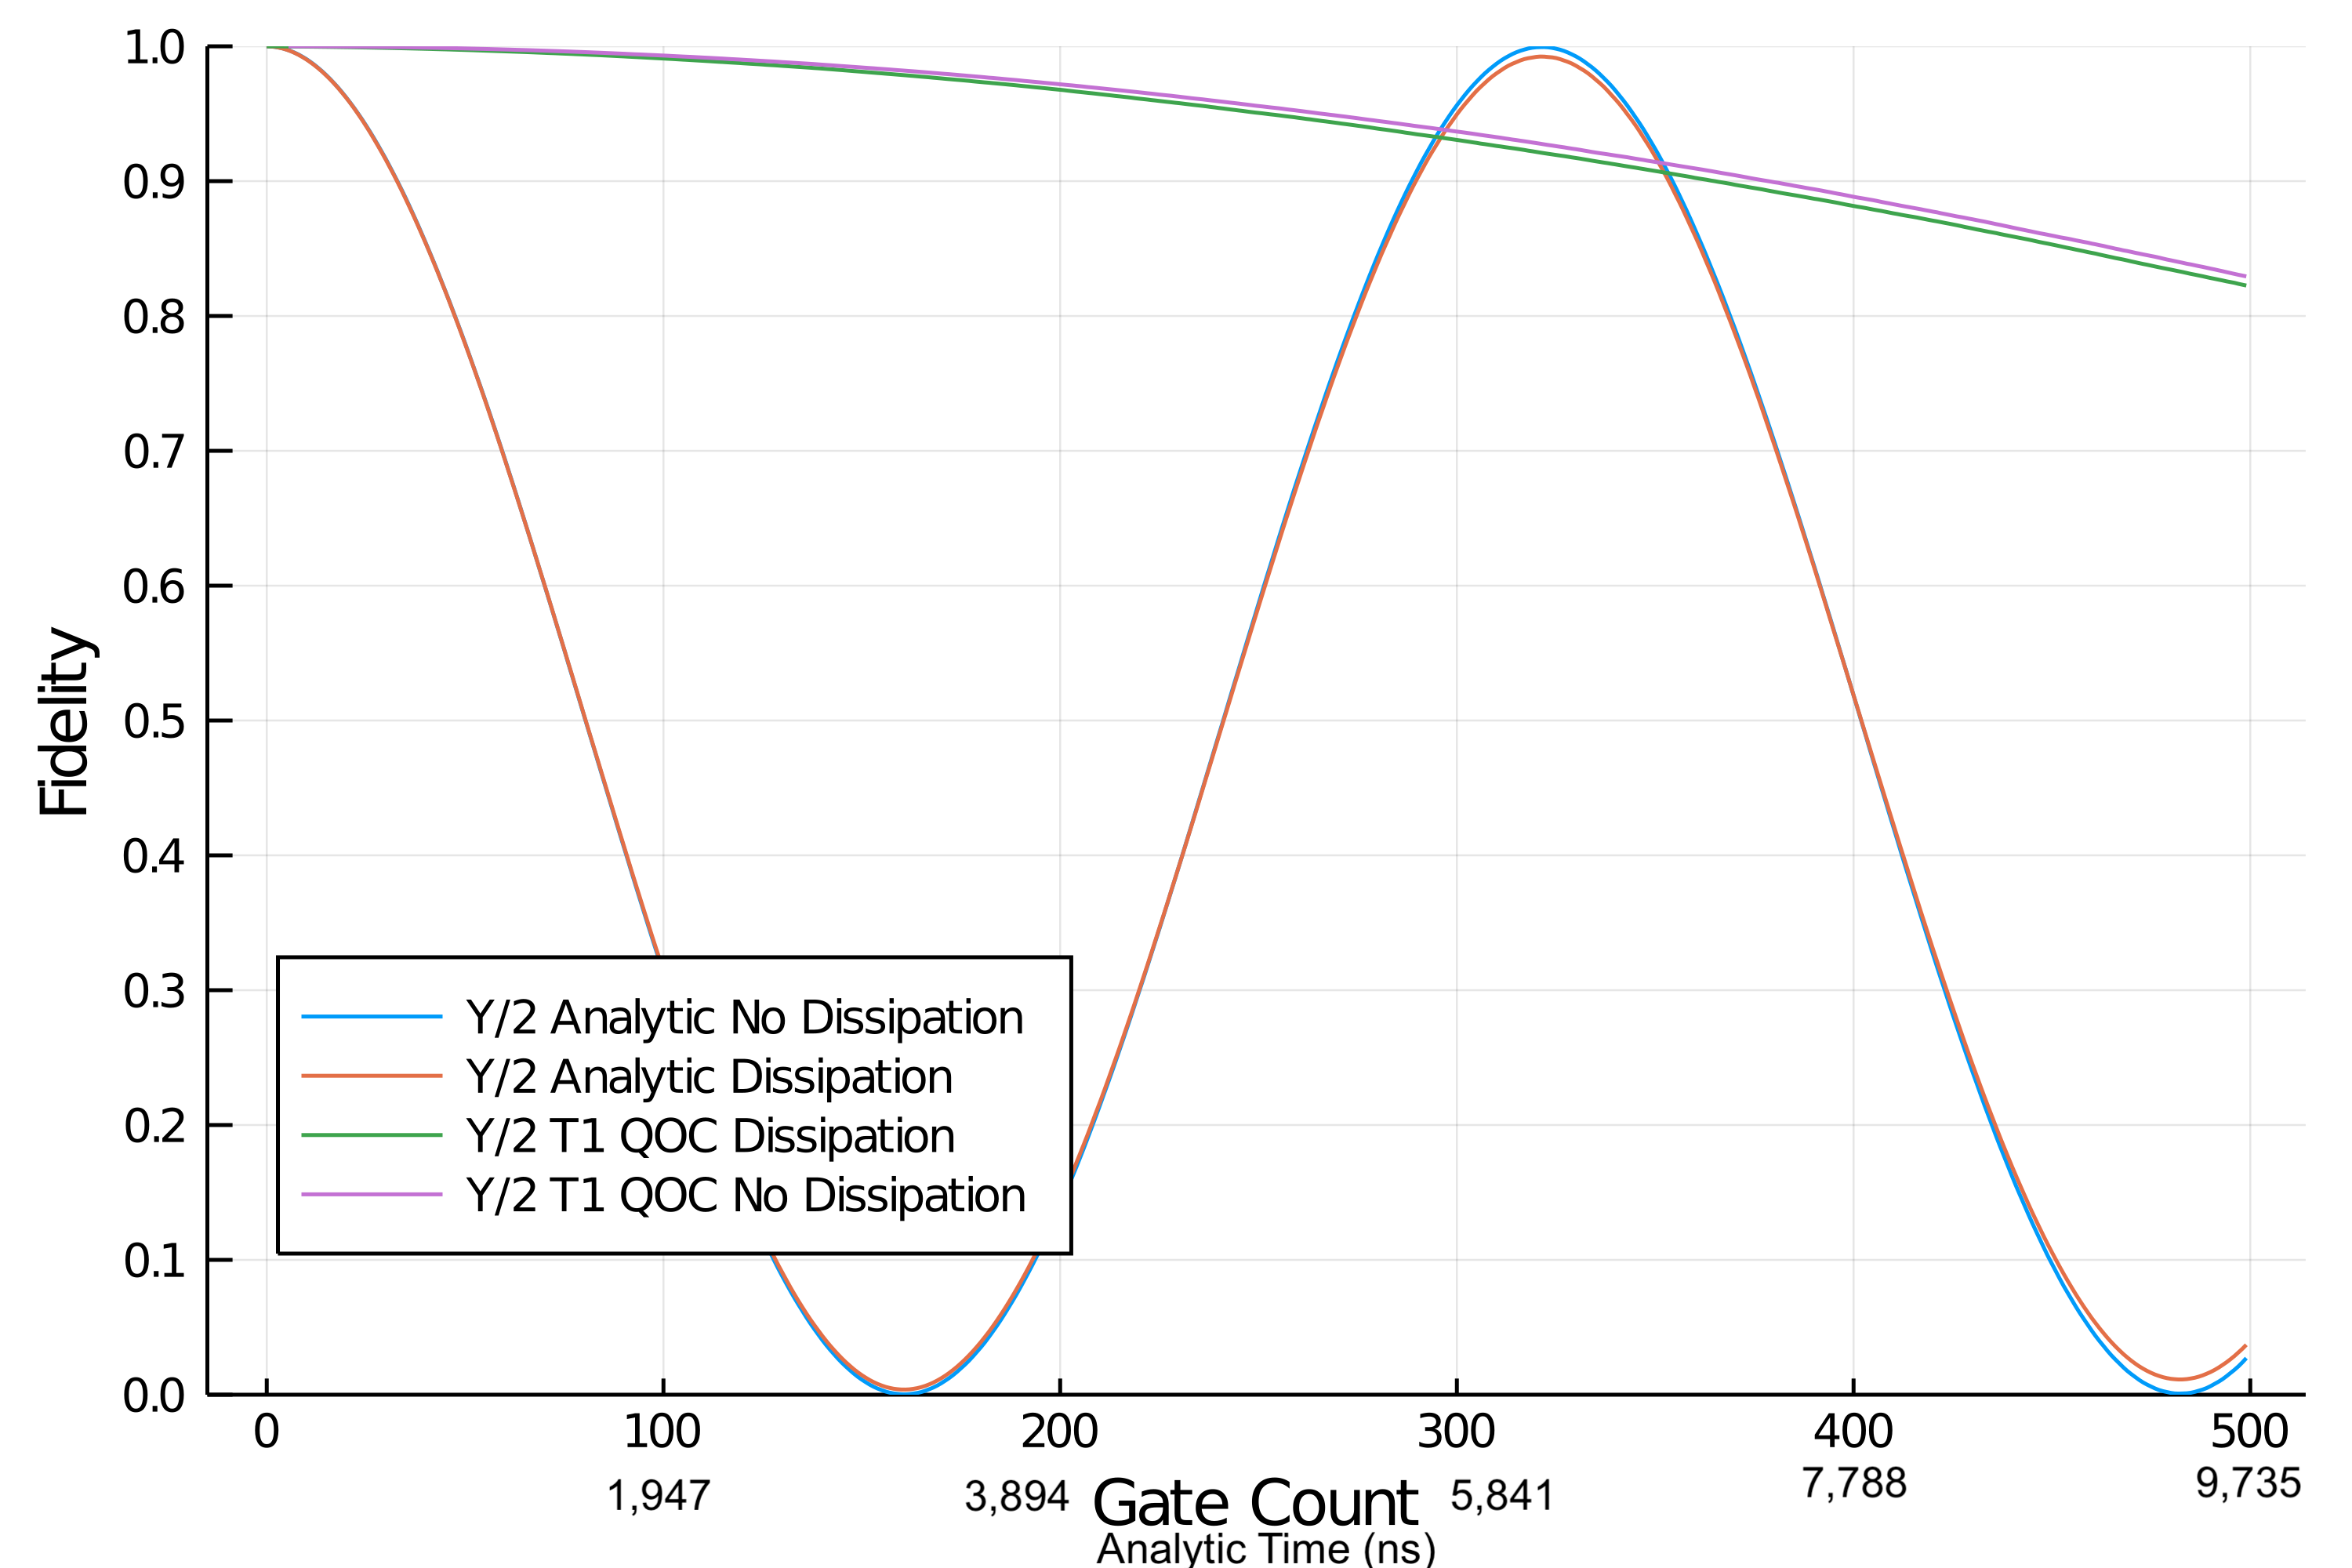
\includegraphics[width=\linewidth]{assets/00045_spin16.png}
    \label{fig:sub-first}
  \end{subfigure}
  \begin{subfigure}{.33\textwidth}
    %% 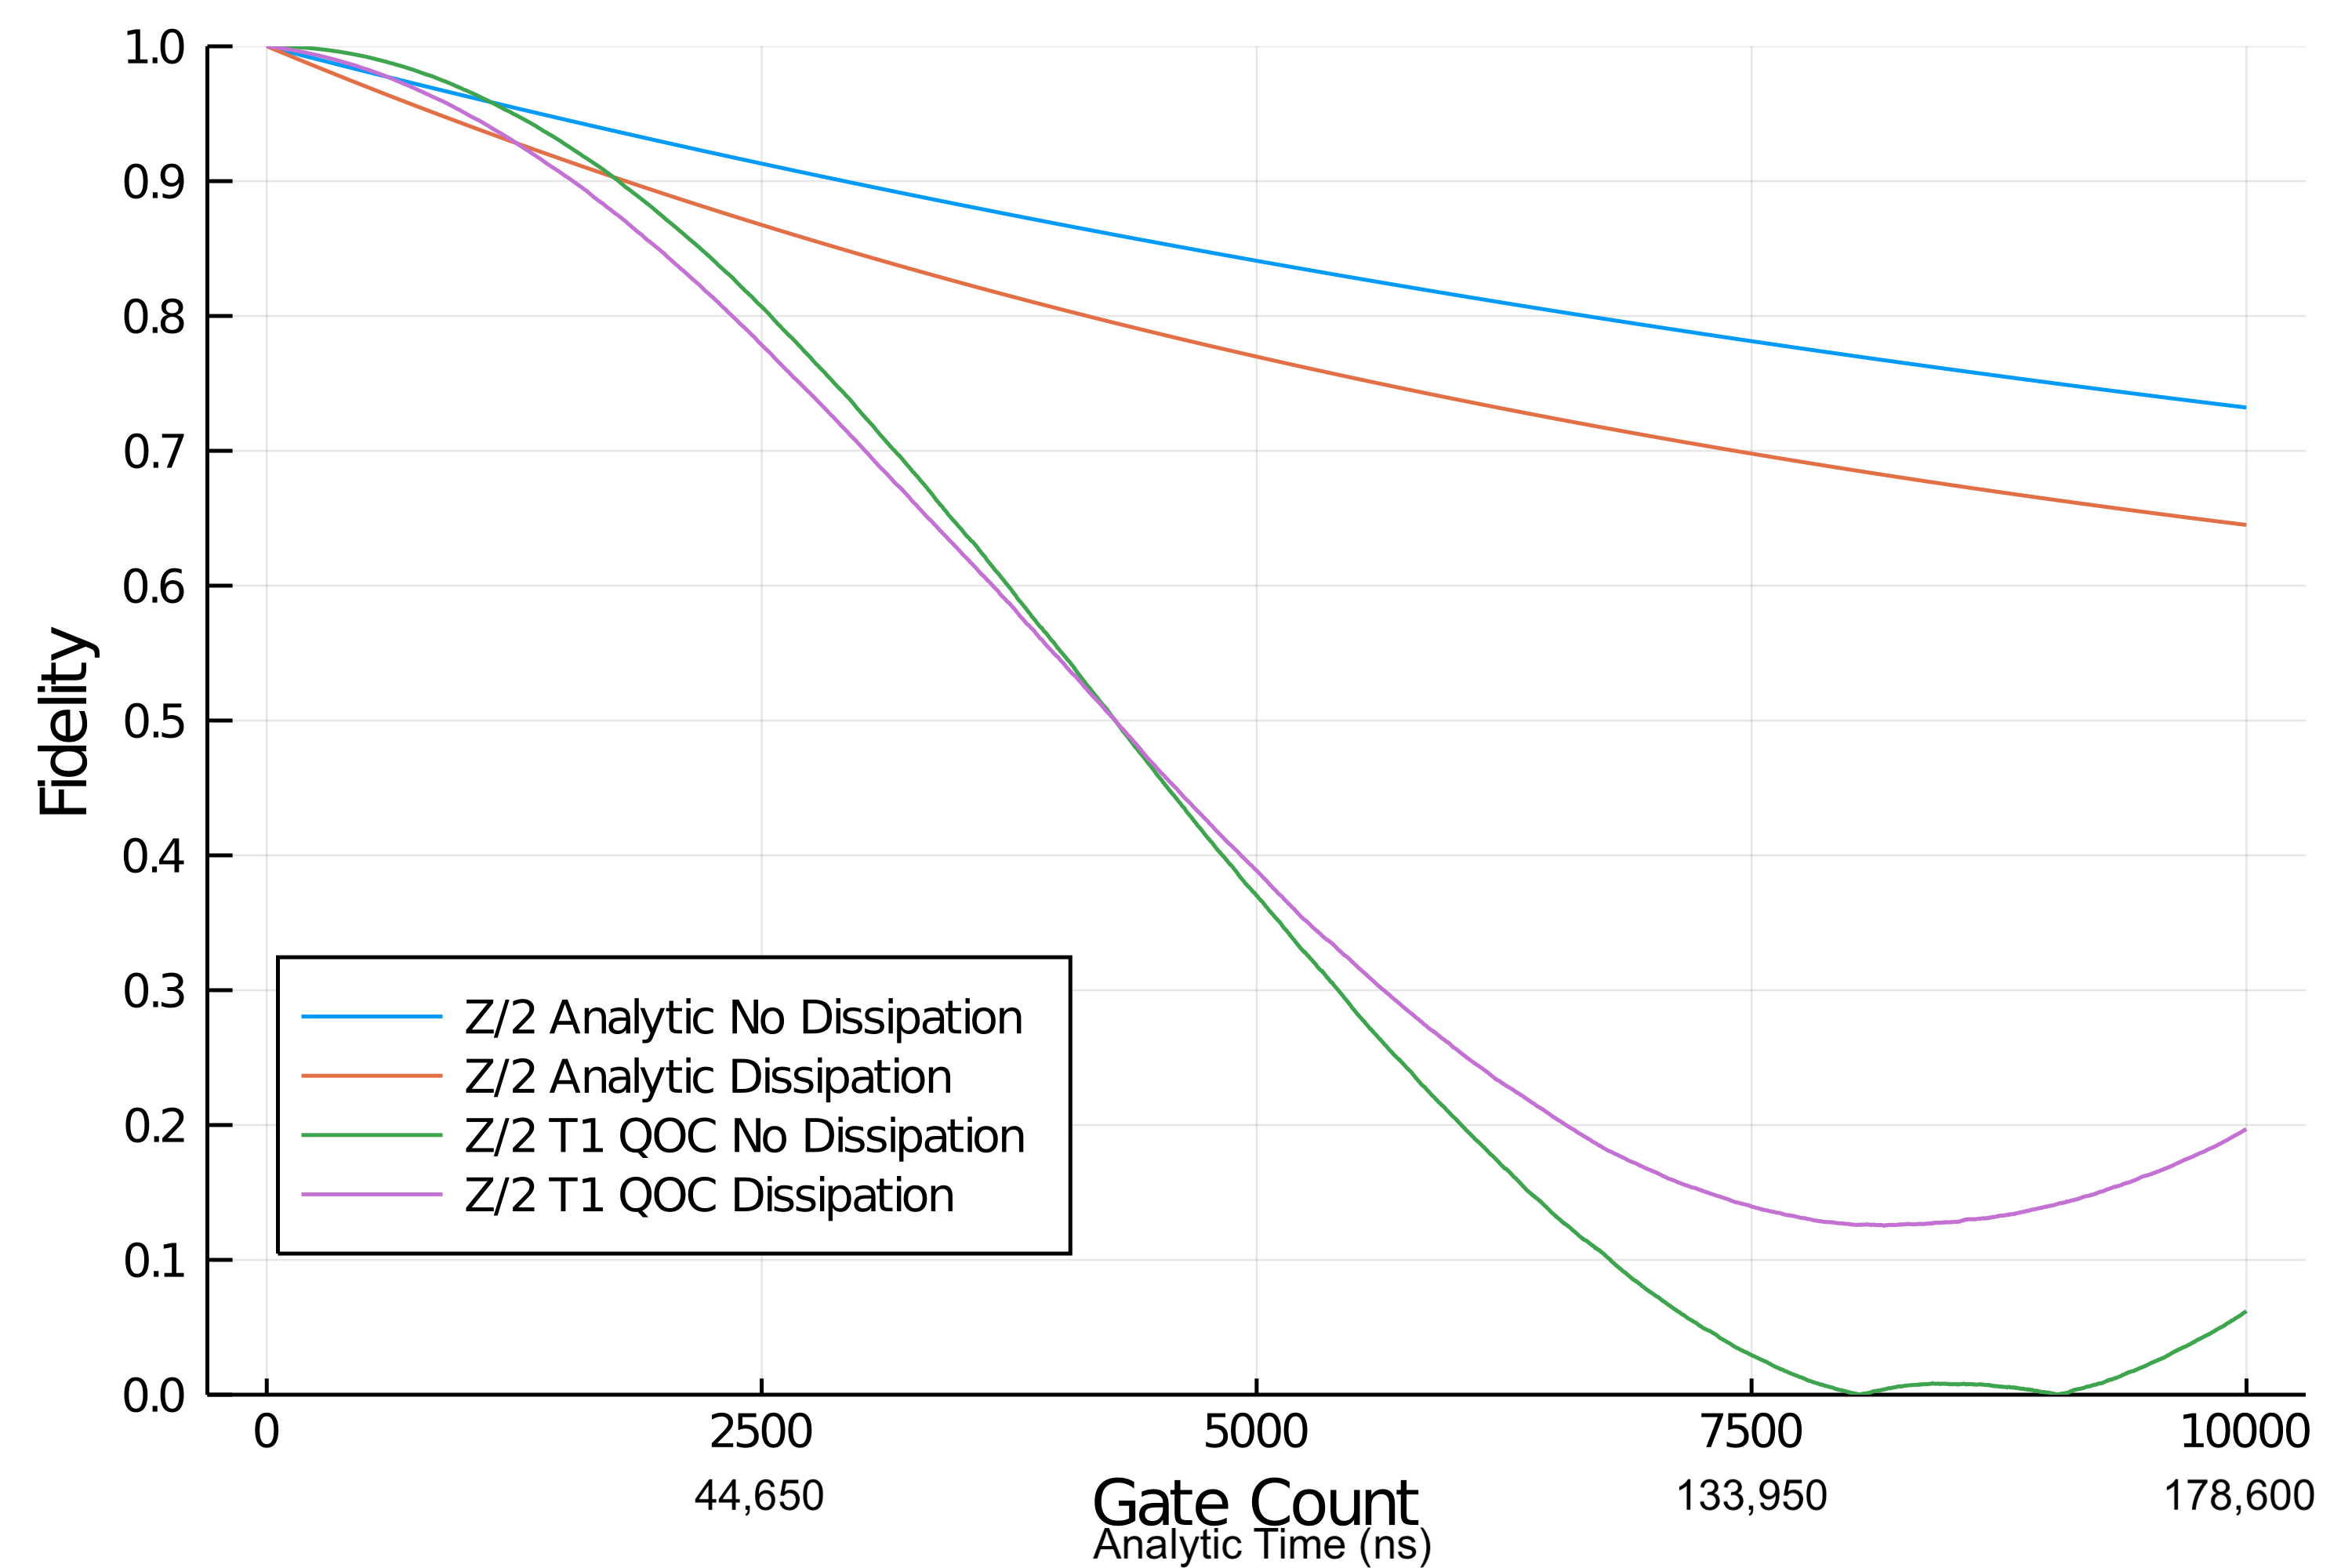
\includegraphics[width=\linewidth]{assets/00047_spin16.png}
    \label{fig:sub-second}
  \end{subfigure}
  \begin{subfigure}{.33\textwidth}
    %% 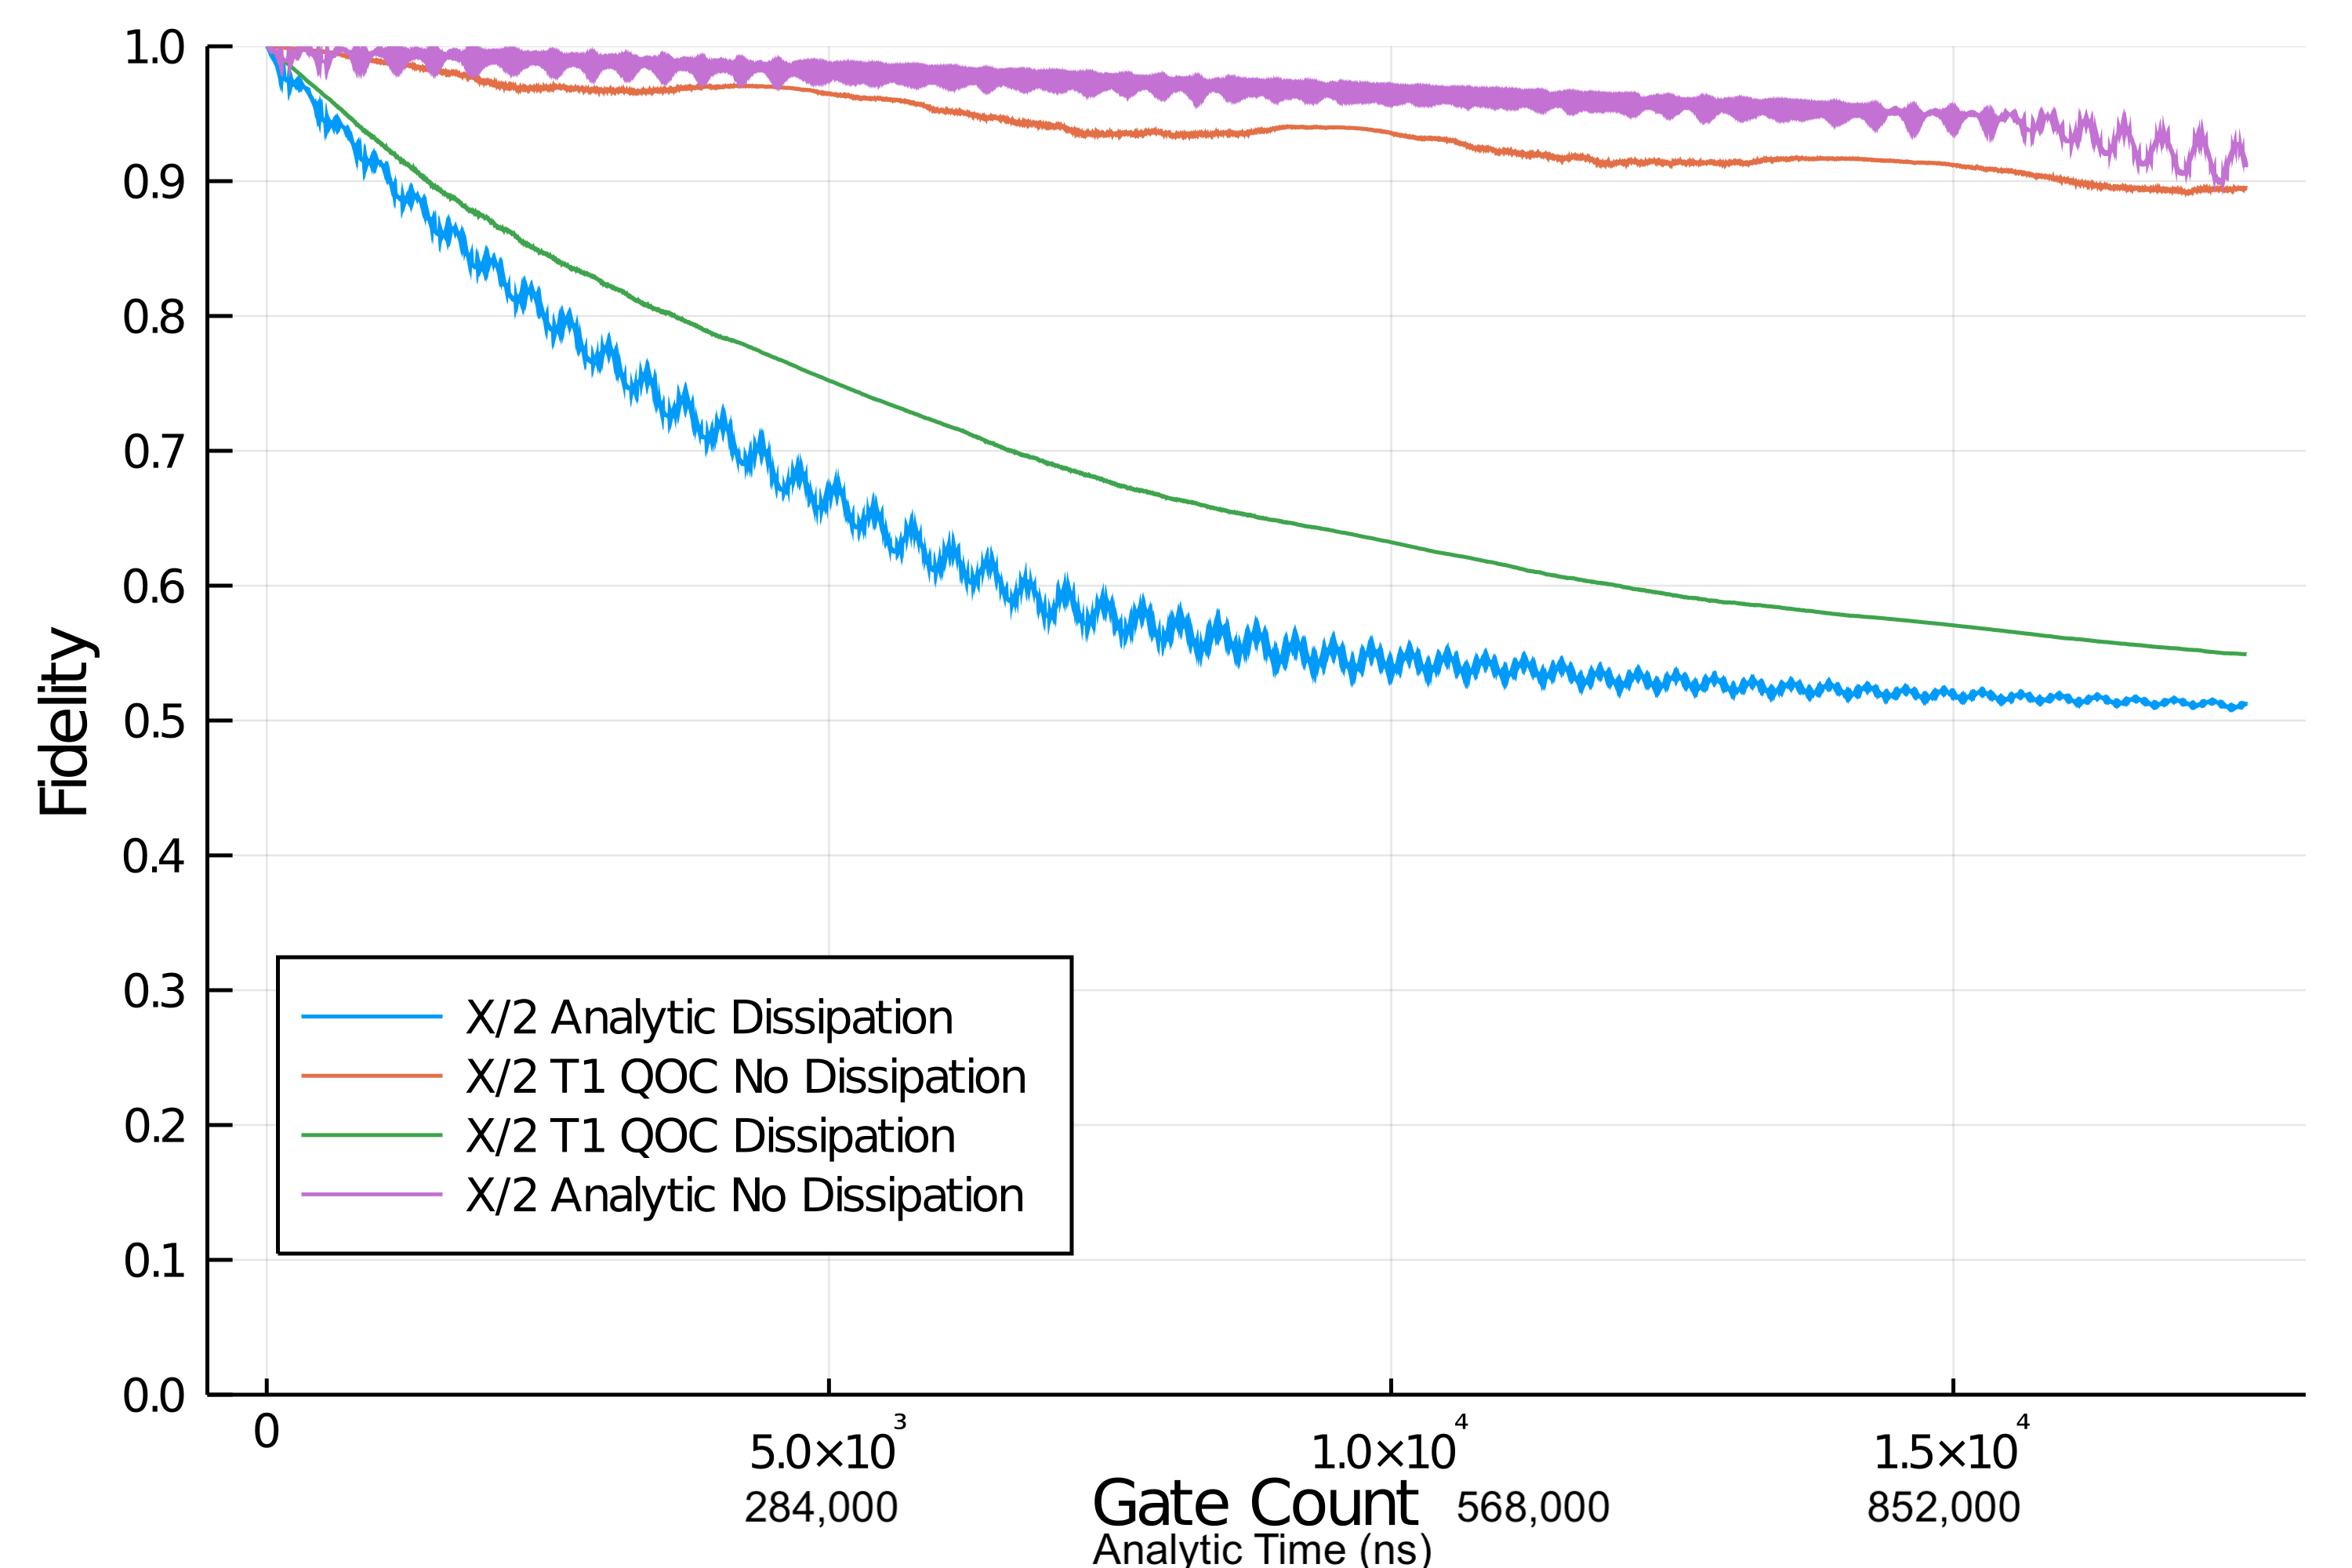
\includegraphics[width=\linewidth]{assets/00049_spin16.png}
    \label{fig:sub-third}
  \end{subfigure}
  \caption{Master equation simulation with $T_{1}$ dissipation for all basis gates.}
  \label{fig:fig}
\end{figure}


%% SECTION 5
\section{Robustness to $T_{\phi}$-type Noise}
(Strategy) System parameter deviations arise due to
measurement error and noise injection. For example,
we might measure $\omega_{q}$ inaccurately,
which leads to a deviation from
the the drive frequency $\omega_{d}$.
Further, we may have some temperature dependent gain
in the lines leading to the device, or 1/$f$ noise
and $A(\Phi_{\textrm{ext}})$ comes out with some
$\delta A$ on the flux axis.
Both of these effects lead to dephasing,
uncertain dynamics, and thus erroneous computation.

These problems are typically attacked with dynamic decoupling
sequence where an erroneous rotation is compensated for with
one that cancels the $\delta$. However, we can do better
than the first order variants of these pulses.

We propose two methods for engineering robustness
to system parameter deviations. The first we call the
derivative method. We use the intuition that
making the final state insensitive to changes
in the system parameter is encoded in the derivative
$\partial_{\omega}^{l} \ket{\psi_{N}}$.
In particular, we find that going to the second
derivative is good. The first derivative is already
small, especially for the $\delta A$ time, because,
near the end of optimization, the
optimizer is unable to improve the final state by
changing the flux bias.
The dynamics for propgating the derivative of the state
are found by differentiating the schroedinger equation
dynamics with respect to the parameter of interest.
The scheme boils down to propagating sequential
derivatives of the parameter you want to be
robust to $\partial_{\omega}^{l}$ and penalizing thier norm
${\lvert \partial_{\omega}^{l} \lvert}^{2}$.

The other scheme we call the sampling method. This method
is well-known in the trajectory optimiztion. In this scheme
we propgate an array of states whose dynamics differ
in that the parameter of interest is altered slightly
for each state. In the 3-point sampling method we
propagate $\psi_{\pm}$, $\psi$ where
$\omega_{\pm} = \omega \pm \delta \omega$. Here $\delta$ is
typically taken at standard deviations of the parameter
of interest.

(Results) We compare the simplest schemes
for the derivative and sampling methods to
the CORPSE dynamic decoupling sequence.
They perform X better by Y metric.

We also find that longer gate durations allow for
greater robustness.

%% F5.1
%% TODO: Update this and make sure it is for X/2.
%% I'm not sure if we should include all gates Z/2, Y/2, X/2
%% because I don't know what the dynamic decoupling analogy
%% for Z/2 and Y/2 are. On the other hand we would
%% want to include all of them to show that the benefit
%% is not uniform across gates.
\begin{figure}
  %% 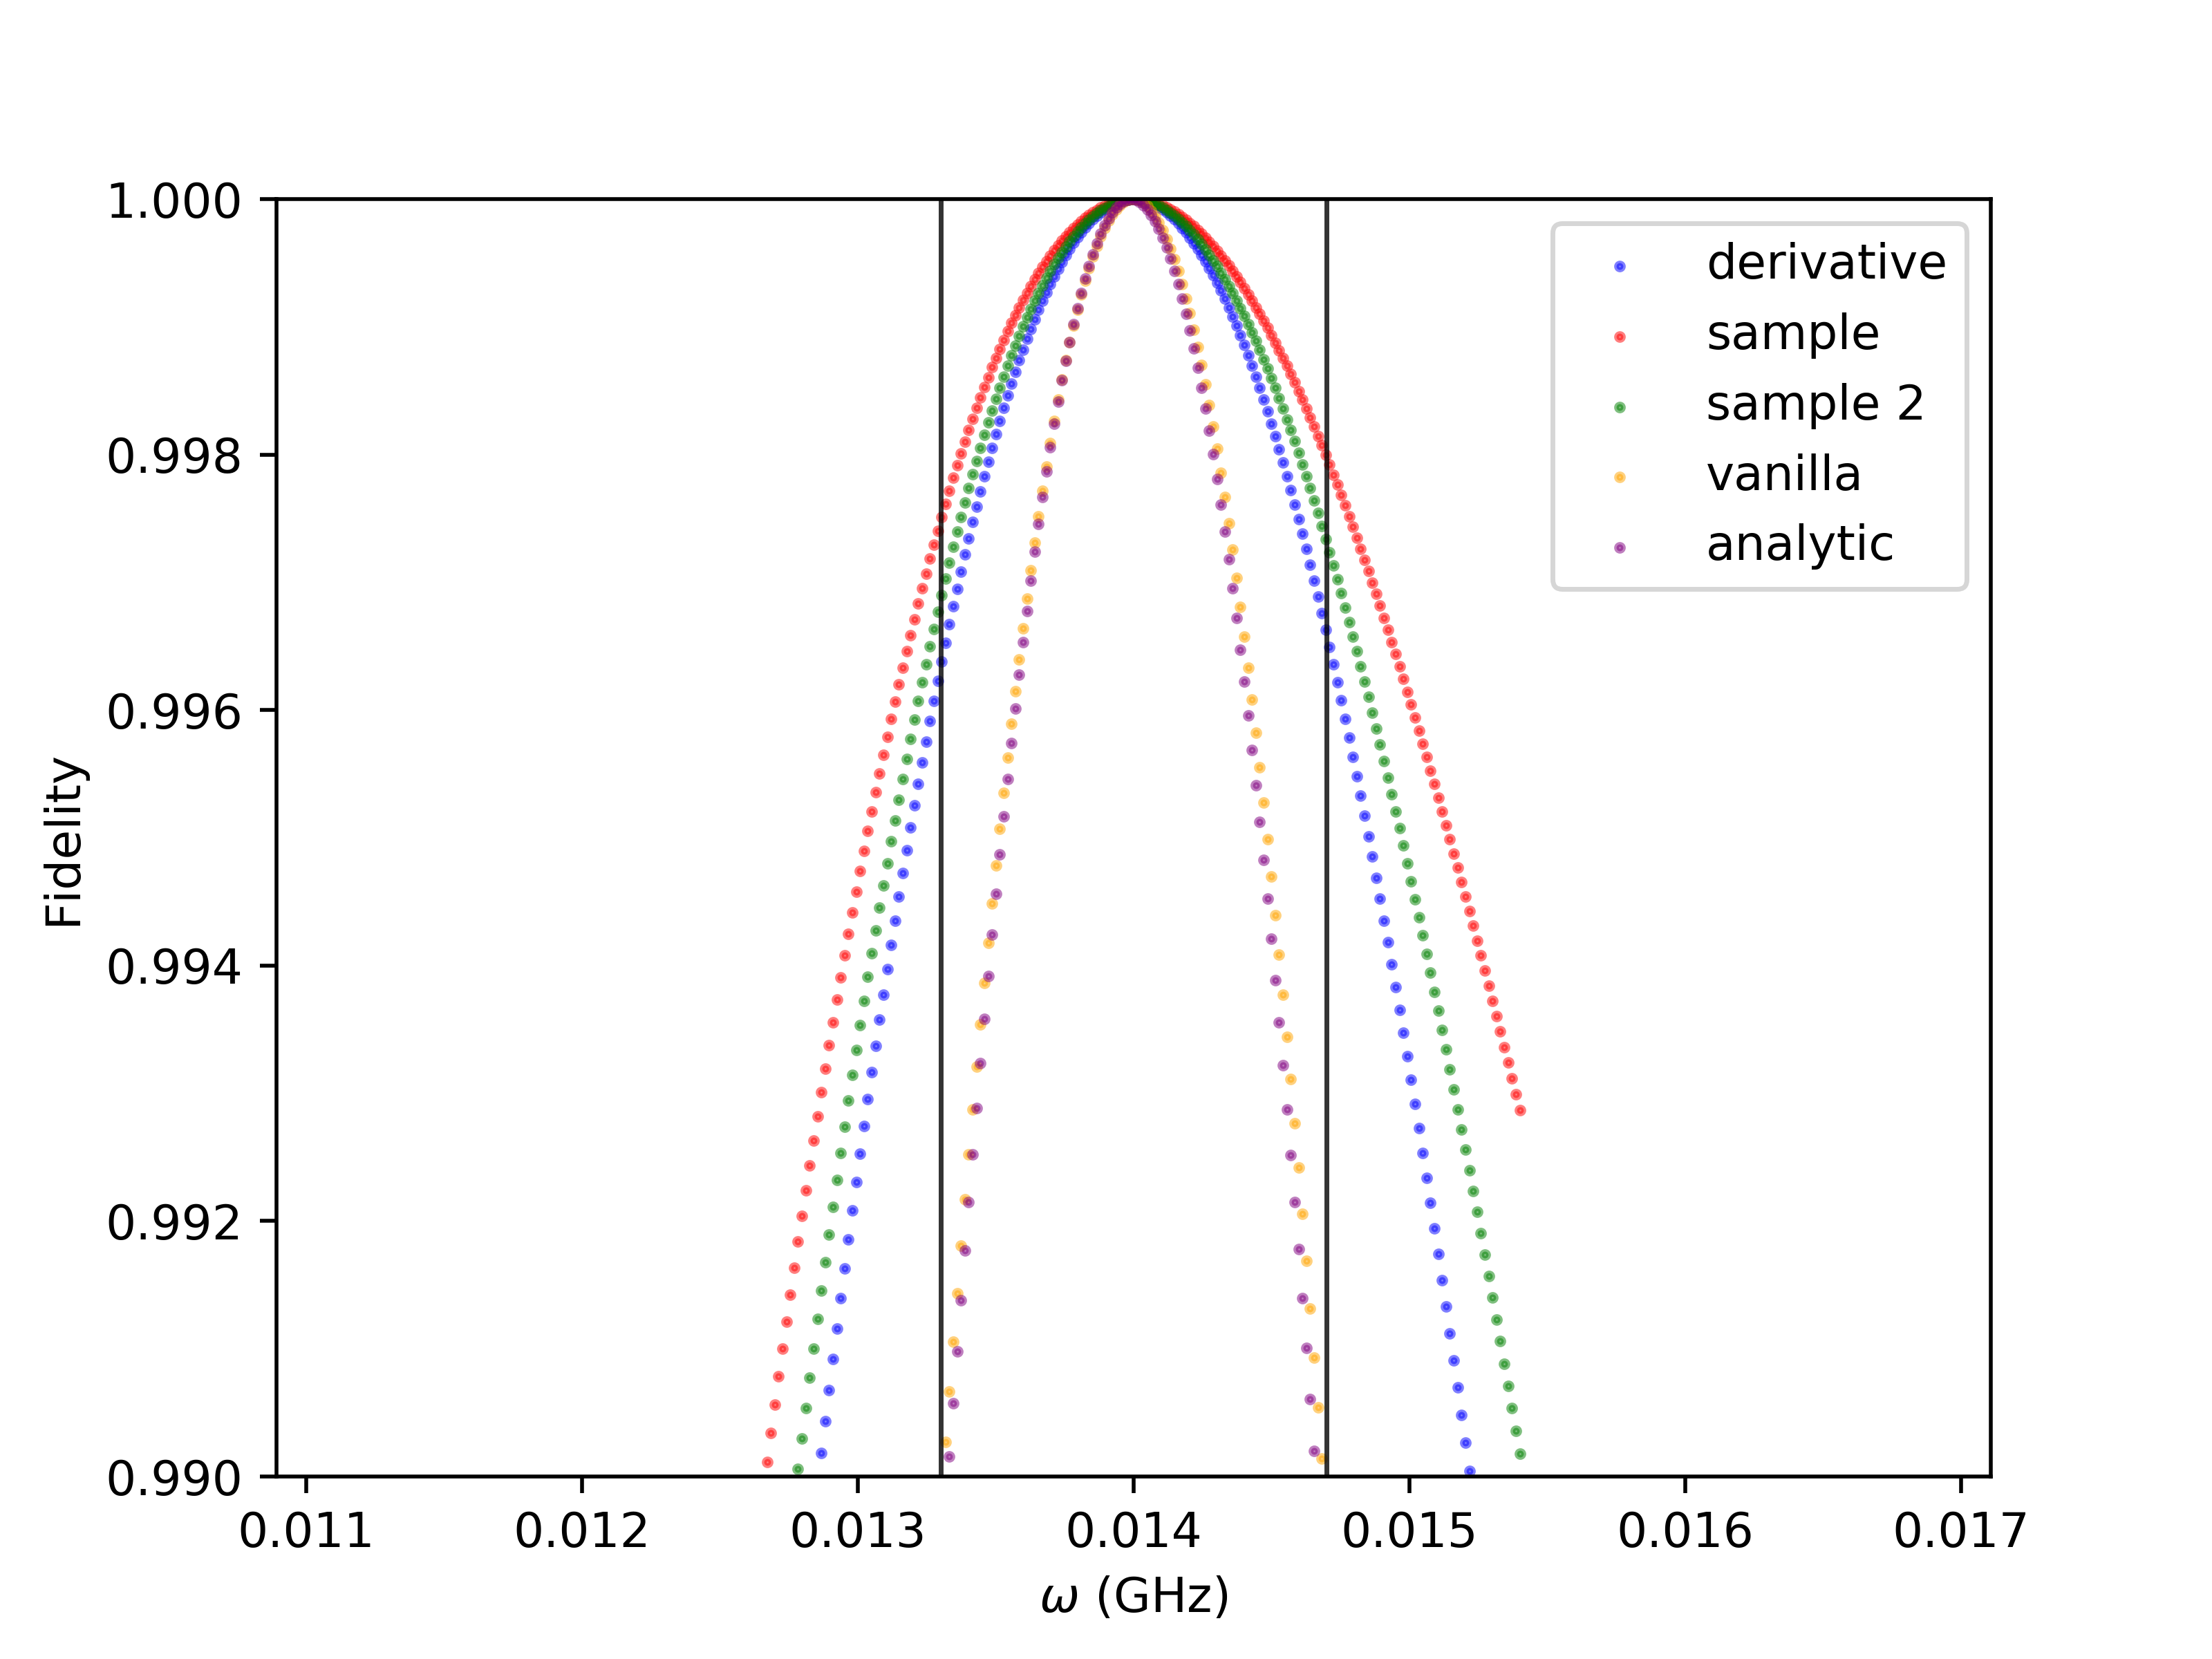
\includegraphics[width=\linewidth]{assets/00005_spin12_hpsweep.png}
  \caption{fidelity v.s. $\omega$ for the $X/2$ gate via
    analytic, 3-sample, 2-derivative (maybe add 5-sample and 3-derivative)}
\end{figure}

%% F5.2
%% TODO: Update this and make sure it is for X/2.
%% Add inset to show high-performing variants at large time steps.
\begin{figure}
  %% 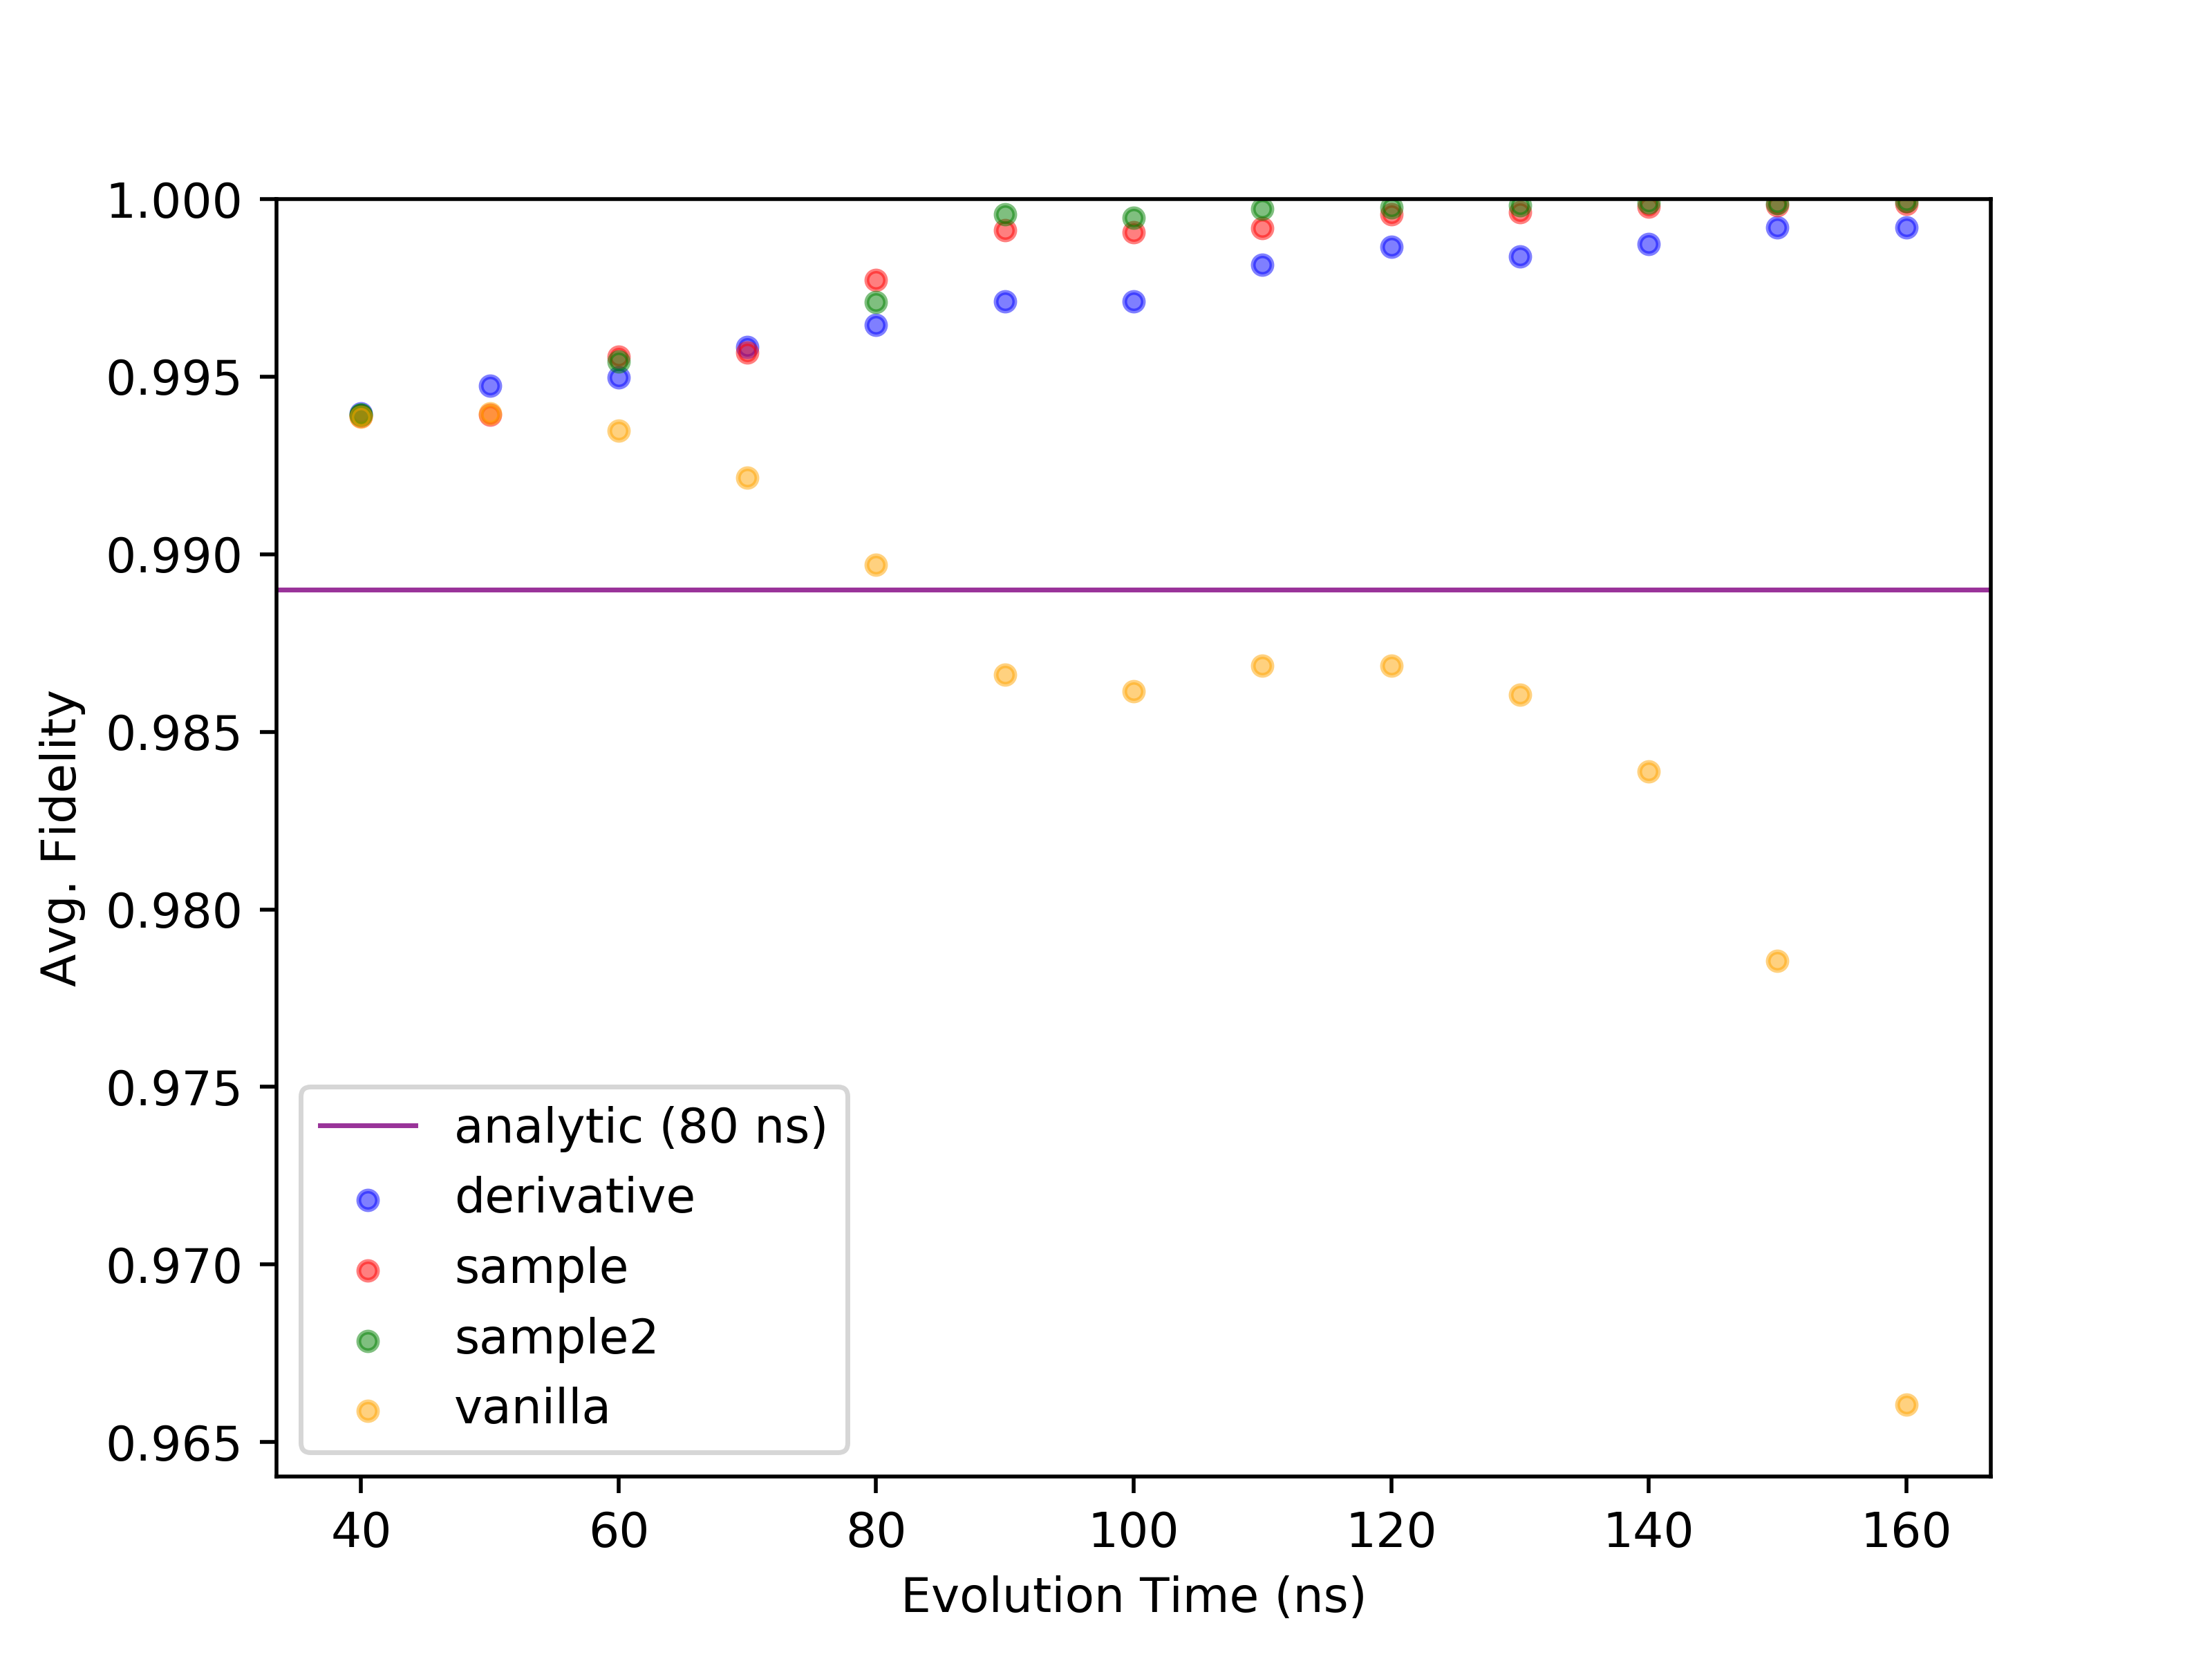
\includegraphics[width=\linewidth]{assets/00006_spin12_hpsweep.png}
  \caption{fidelity at $\omega \pm \sigma_{\omega}$ v.s. time for the
    $X/2$ gate via analytic, 3-sample, 2-derivative
    (maybe add 5-sample and 3-derivative)}
\end{figure}

%% F5.3
%% TODO: Make this figure. My guess is we want a 5-sample, with 2 at \omega_{\pm}
%% and 2 at A_{\pm} as well as 2-derivative of both parameters separately.
\begin{figure}
  %% 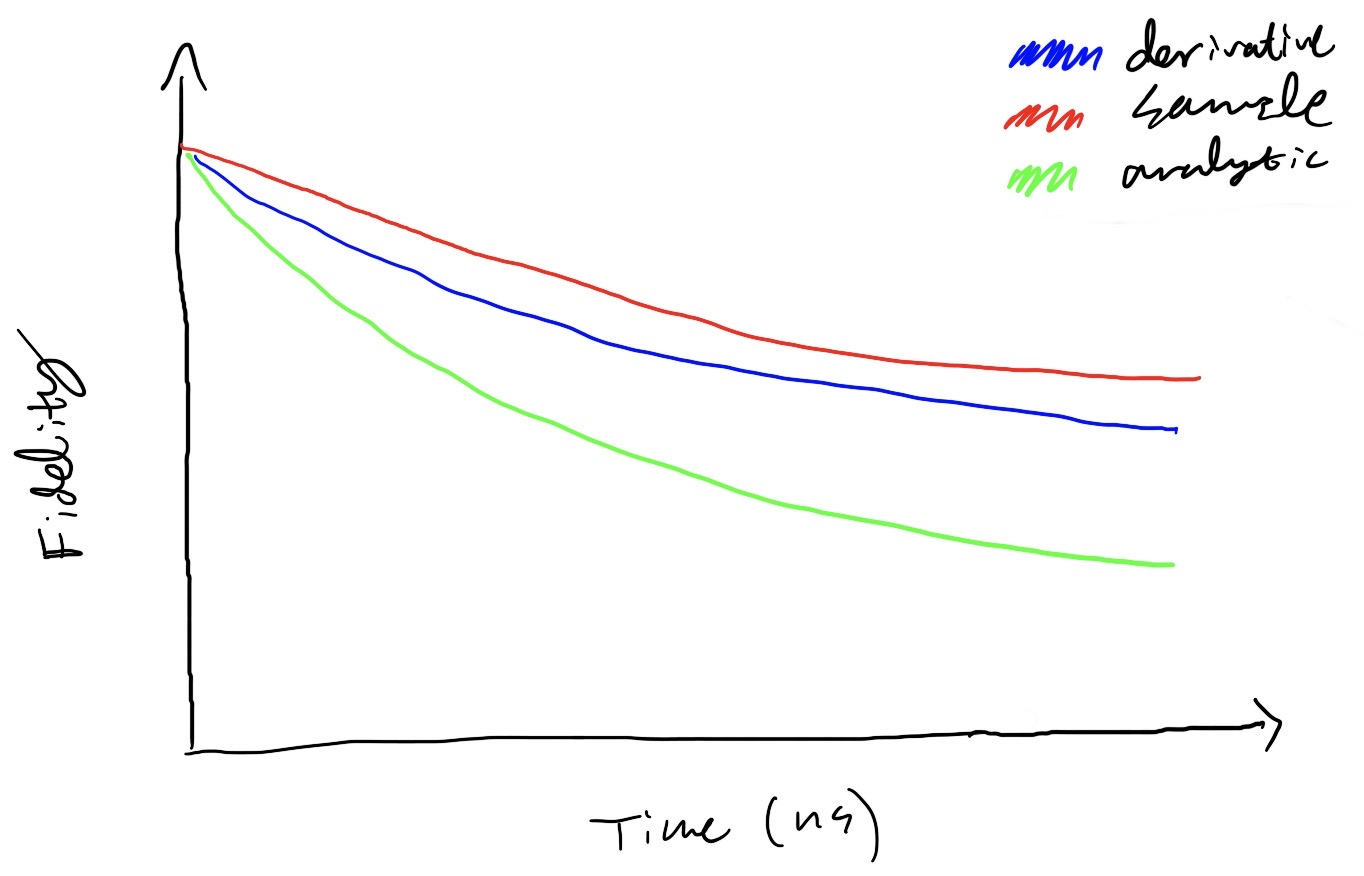
\includegraphics[width=\linewidth]{assets/t2_temp.jpg}
  \caption{Master equation simulation with $T_{2}$ dissipation
    comparing the gates robust to $\delta \omega_{q}$ and $\delta A$ against
    the analytic gate.}
\end{figure}


%% TODO: Fig: Full ME simulation for best T1 and T\phi pulses
%% v.s. analytic

%% SECTION 6
\section{Discussion}
We have proposed some schemes and they work well.


\appendix
%% APPENDIX 1
\section{Ricatti Recursion}
This will give the reader unfamiliar with trajectory
optimization intuition for how the trajectory optimization
update scheme works and why it is better than
a more naive method.


%% APPENDIX 2
\section{Measurements}
We measure $T_{1}$ using the standard experiment
and $T_{2}$ using te Ramsey experiment. We fit with splines
and the data looks like fig. 3 in Helin's paper \cite{zhang2020universal}.
We measure $\omega_{q}$ and $\sigma_{\omega_{q}}$ using X method.


%% APPENDIX 3
\section{ME Simulation}
We model dissipation using the lindblad master
equation and standard collapse operators for
longitudinal relaxation and dephasing
of a two-level system.


%% APPENDIX 4
\section{Derivative Method}
\begin{equation}
  \begin{aligned}
    \partial_{\omega}^{2} \partial_{t} \psi
    = \frac{-i}{h} [&2 \cdot \frac{\sigma_{z}}{2} \partial_{\omega} \psi\\
      &+ (\omega \frac{\sigma_{z}}{2} + A \frac{\sigma_{x}}{2}) \partial_{\omega}^{2} \psi]
  \end{aligned}
\end{equation}


\bibliography{refs}

\end{document}
